\section{Theory}

\subsection{Calculating Resolution as Function of Height}

If one knows the resolution of the camera, the height from which the photo was
taken and the angle of view of the camera, then one can calculate the resolution
of the resulting photographs, in terms of how many meters correspond to a single
pixel.

To do this, the geometry of the situation, illustrated in Figure
\ref{fig:resolution-views}, is parametrised as follows:

\begin{itemize}
    \item Distance photographed along ground: $x$ and $y$
    \item Resolution of camera (n\# pixels): $r_x$ and $r_y$
    \item Height from which photo was taken: $h$
    \item Angle of view of camera: $\alpha_x$ and $\alpha_y$
    \item Number of meters corresponding to a single pixel: $\mu_x$ and $\mu_y$
\end{itemize}

\begin{figure}
    \begin{center}
        \begin{subfigure}[b]{0.49\textwidth}
            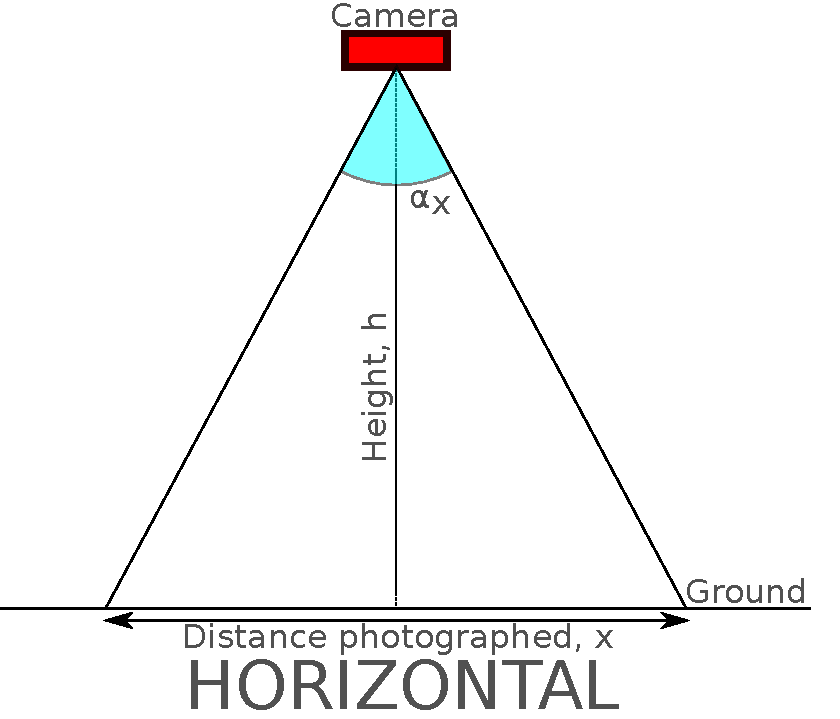
\includegraphics[width=\textwidth]{HorizontalView}
            \caption{The horizontal view of the angle of view of the camera
            facing the ground.}
            \label{subfig:horizontal-view}
        \end{subfigure}
        \begin{subfigure}[b]{0.49\textwidth}
            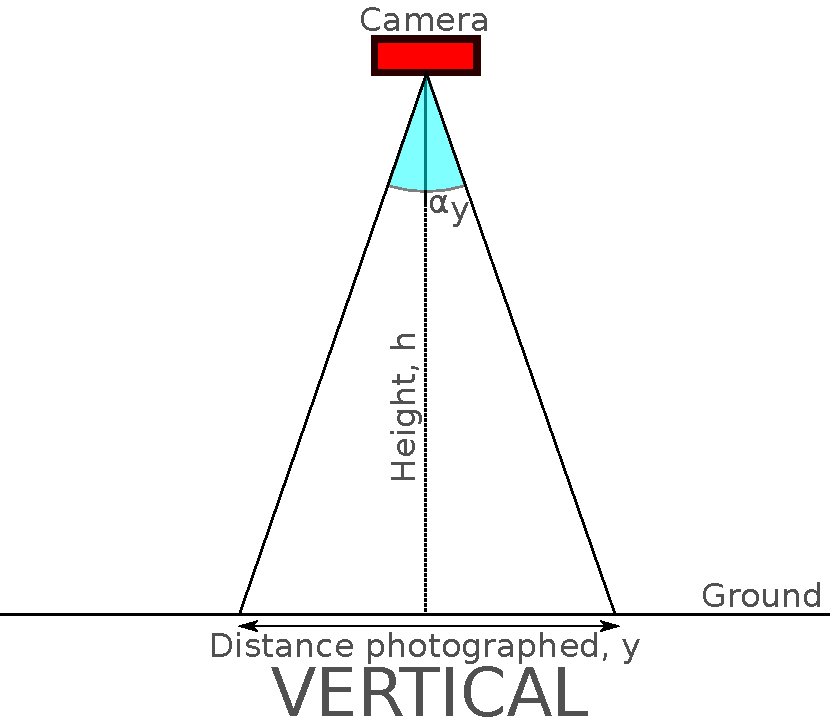
\includegraphics[width=\textwidth]{VerticalView}
            \caption{The vertical view of the angle of view of the camera facing
            the ground.}
            \label{subfig:vertical-view}
        \end{subfigure}
        \caption{The views of the angle of view as the camera faces directly
        towards the ground.}
        \label{fig:resolution-views}
    \end{center}
\end{figure}

Then according to this parametrisation, as a matter of elementary trigonometry:

\begin{align}
    \tan\left(\frac{\alpha_x}{2}\right) &= \frac{x}{2h} ~\mathrm{and} \\
    \tan\left(\frac{\alpha_y}{2}\right) &= \frac{y}{2h} \\
\end{align}

Rearranging this for $x$ and $y$ gives:

\begin{align}
    x &= 2h\tan\left(\frac{\alpha_x}{2}\right) ~\mathrm{and} \\
    y &= 2h\tan\left(\frac{\alpha_y}{2}\right)
\end{align}

Then the resolution in meters per pixel is simply this distance $x$ divided by
the total number of pixels in the photograph:

\begin{align}
    \mu_x &= \frac{x}{r_x} = \frac{2h\tan\left(\frac{\alpha_x}{2}\right)}{r_x}
    ~\mathrm{and} \\
    \mu_y &= \frac{y}{r_y} = \frac{2h\tan\left(\frac{\alpha_y}{2}\right)}{r_y}
\end{align}

This agrees approximately with the values generated by PhotoScan in doing the
photogrammetric reconstruction, discussed in Sections
\ref{sec:results/long-ashton/with-gcps} and
\ref{sec:results/avon-gorge/with-gcps}.

\subsection{Ensuring sufficient photo overlap}

Agisoft states in the PhotoScan User Manual\footnote{PhotoScan 1.0.0 user
Manual, ``Capturing Scenarios'', Page 5.
\url{http://downloads.agisoft.ru/pdf/photoscan-pro\_1\_0\_0\_en.pdf}} that 80\%
overlap is needed for standard front overlap between successive photos. Thus,
one can calculate the speed one needs to travel at to ensure that if one takes
photos every five seconds, the overlap is at least 80\%.

The distance between the photo locations, illustrated in Figure
\ref{fig:overlap}, is then given by:

\begin{align}
    d_{int} &= 2h\tan\left(\frac{\alpha_y}{2}\right) - \mathrm{overlap} \\
            &= 2h\tan\left(\frac{\alpha_y}{2}\right) -
                   2h\omega\tan\left(\frac{\alpha_y}{2}\right) \\
            &= 2h\tan\left(\frac{\alpha_y}{2}\right)\left[ 1 - \omega \right]
\end{align}

\begin{wrapfigure}{r}{0.5\textwidth}
    \centering
    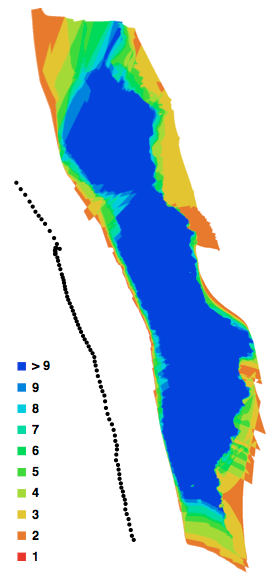
\includegraphics[width=0.5\textwidth]{Overlap}
    \caption{An illustration of the overlap between successive photos, and the
    distance between each photo.}
    \label{fig:overlap}
\end{wrapfigure}

Where $d_{int}$ is the required maximum distance between the photos needed to
ensure an overlap of $\omega$, where the vertical angle of view is $\alpha_y$
and the photographs are taken from a height $h$.  For the Ixus 132 we used with
$\alpha_y = 48.9^{\circ}$, requiring an overlap of $\omega = 0.8$ gives:

\begin{equation}
    d_{int} = 0.182h ~\mathrm{meters/second}
\end{equation}

If the photos are taken once every five seconds ($ t_{int} = 5 $ seconds), as we
did, then this gives a maximum UAV velocity of:

\begin{equation}
    v_{UAV} = \frac{d_{int}}{t_{int}} = 0.0364h ~\mathrm{meters/second}
\end{equation}

Taking a reasonable height of $ h = 50 $ meters thus gives:

\begin{equation}
    v_{UAV} = 1.82 ~\mathrm{meters/second}
\end{equation}

This is a very reasonable and achievable speed.
